\documentclass{standalone}

\usepackage{tikz}

\begin{document}
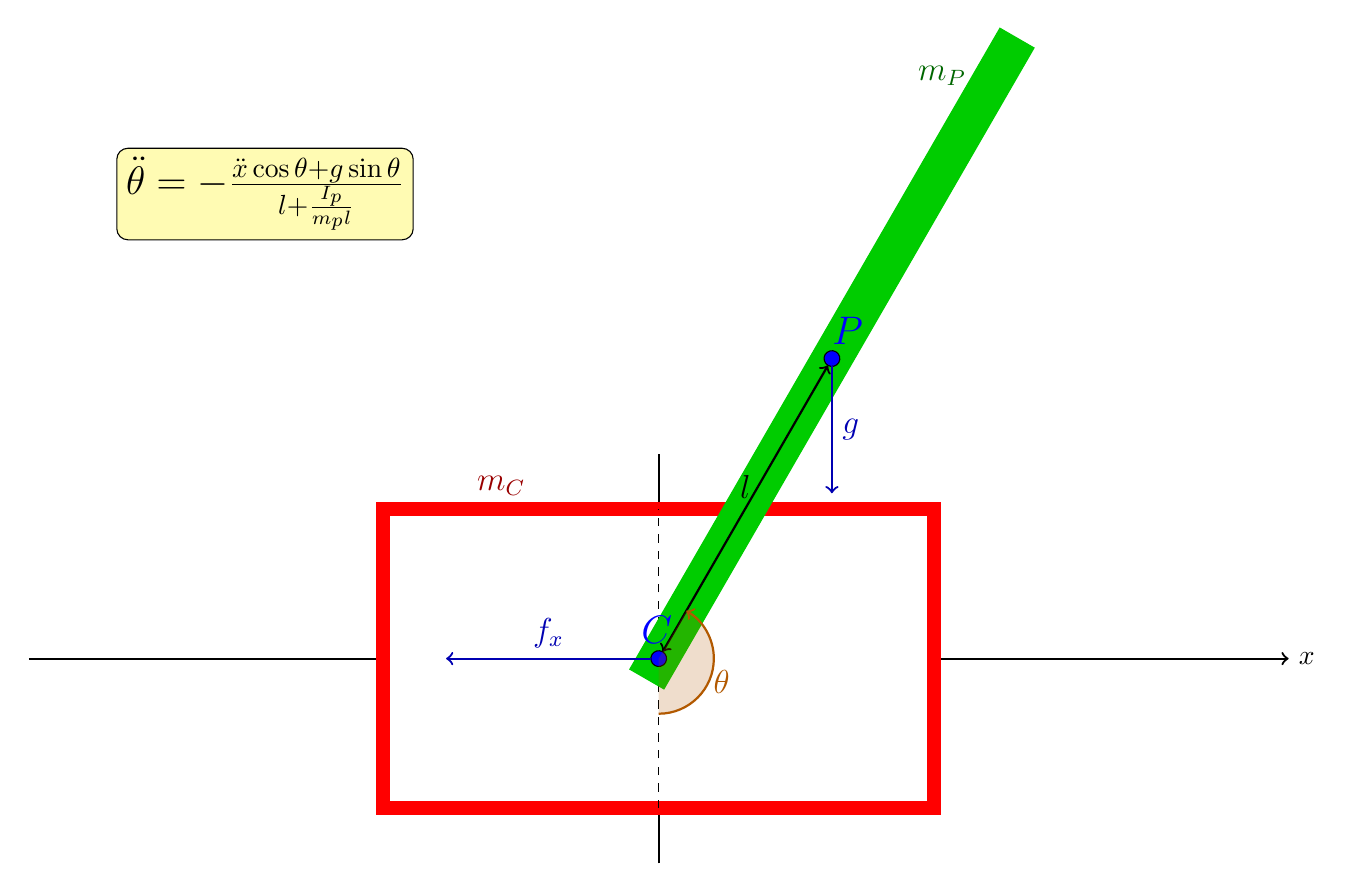
\begin{tikzpicture}
    % world
    \draw[->, thick] (-1,3.1) -- (15,3.1) node[right] {\(x\)};
    \draw[-, thick] (7,0.5) -- (7,5.7);

    % hull
    \filldraw[red!100!black, fill=white, line width=5] (3.5,1.2) rectangle (10.5,5.0);

    % y axis help
    \draw[-, dashed] (7,1.2) -- (7,5.0);

    % stick
    \begin{scope}[rotate around={150:(7, 3.1)}]
        \filldraw[green!80!black, fill=green!80!black] (6.75, 3.4) rectangle (7.25, -6);

        % C
        \filldraw[fill=blue] (7, 3.1) circle [radius=0.1];
        \draw[blue] (7.2, 2.8) node {\Large \(C\)};

        % P
        \filldraw[fill=blue] (7, -1.3) circle [radius=0.1];
        \draw[blue] (7, -1.7) node {\Large \(P\)};

        % l
        \draw[<->, thick, black] (7,3) -- (7, -1.2) node[midway,above] {\large \(l\)};
    \end{scope}

    % f_x
    \draw[<-, thick, blue!70!black] (4.3,3.1) -- (6.9, 3.1) node[midway,above] {\large \(f_x\)};

    % g
    \draw[->, thick, blue!70!black] (9.2, 6.81) -- (9.2, 5.2) node[midway,right] {\large \(g\)};

    % \theta
    \draw[->, thick, orange!70!black] (7, 2.4) arc [start angle=-90, end angle=60, radius=0.7];
    \fill[->, opacity=0.2, orange!70!black] (7, 3.1) -- (7, 2.4) arc [start angle=-90, end angle=60, radius=0.7];
    \draw[thick, orange!70!black] (7.8, 2.8) node {\large \(\theta\)};

    % m_C
    \draw[red!60!black] (5, 5.3) node {\large \(m_C\)};

    % m_P
    \draw[green!40!black] (10.6, 10.5) node {\large \(m_P\)};

    % formula
    \draw (2,9) node[fill=yellow!30, draw, rounded corners] {\Large \(\ddot{\theta} = - \frac{\ddot{x} \cos \theta + g \sin \theta}{l + \frac{I_p}{m_pl}}\)};
\end{tikzpicture}
\end{document}